\documentclass[tikz,border=5mm]{standalone}
\usepackage{tikz}
\begin{document}
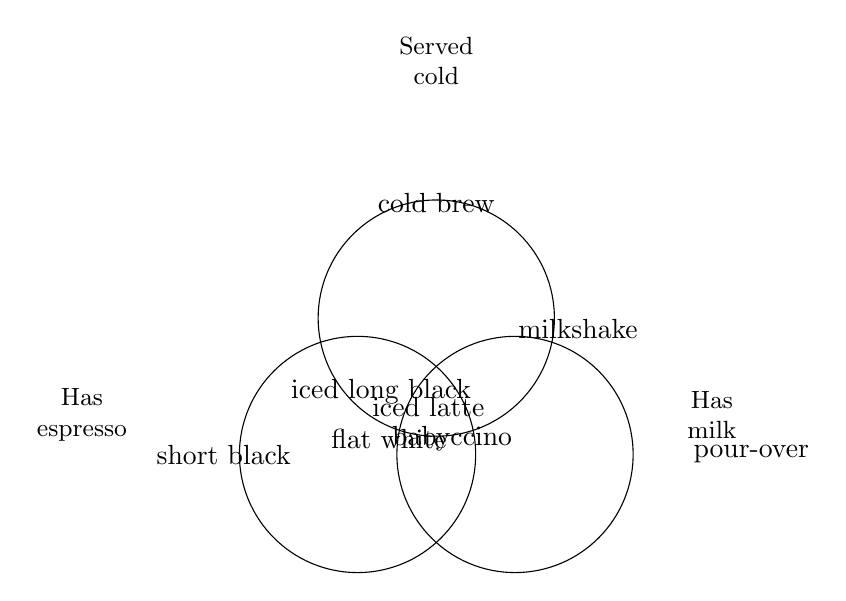
\begin{tikzpicture}[scale=1]
% Parameters
\def\radius{1.5}
\def\dist{2}
% Circle centers (equilateral triangle)
\coordinate (A) at (0,0);
\coordinate (B) at (\dist,0);
\coordinate (C) at (1, 1.732);
% Draw circles
\draw (A) circle (\radius);
\draw (B) circle (\radius);
\draw (C) circle (\radius);
% Circle labels (outside circles)
\node[align=center, font=\small] at (-3.5,0.5) {Has\\espresso};
\node[align=center, font=\small] at (4.5,0.5) {Has\\milk};
\node[align=center, font=\small] at (1,5) {Served\\cold};
% Drink placements in appropriate Venn regions
\node at (-1.7,0) {short black};
\node at (0.4,0.2) {flat white};
\node at (1.2,0.2) {babyccino};
\node at (0.3,0.8) {iced long black};
\node at (2.8,1.6) {milkshake};
\node at (0.9,0.6) {iced latte};
\node at (1,3.2) {cold brew};
\node at (5,0) {pour-over};
\end{tikzpicture}
\end{document}